\section{Course Introduction}

\begin{frame}
\frametitle{Course Target}
\scalebox{0.9}
{
	\begin{adjustbox}{max totalsize={.9\textheight},center}
	\smartdiagramanimated[bubble diagram]{Goal,Data\\Management,Distributed\\System,Big Data\\Tools,Coding,Real world\\applications,Databases, DevOps  }
	\end{adjustbox}
}
\end{frame}
%---------------------------------------------------------
%Example of the  command
\subsection{Learning Objectives and Audience}
\begin{frame}[t]
\frametitle{Learning Objectives}
   	\smartdiagramset{
	%descriptive items y sep = 3em,
	module minimum width=5cm,
	description text width={9cm},
%	description font = \scriptsize\sffamily,
%	description title font=\scriptsize\sffamily,
%	module minimum height={.7cm},
%	description title text width={.5cm},
	}
	\begin{adjustbox}{max totalsize={\textheight},center}
			\smartdiagramanimated[descriptive diagram]{
			{Ch.2 ,Simplify the concepts in data management. Understand the data management life-cycle},
			{Ch.3, {Illustrate the basics of distributed systems concepts.}},
			{Ch.4/6, Be familiar with ETL for (batch/steaming) data over distributed systems ex: Hadoop \& Spark.},
			{Ch.6/7, {Apply QA and testing the data.}},
			{Ch.7, {Building real-life examples.}},
		}
		
	\end{adjustbox}
%}

%\resizebox{.8\textwidth}{!}{% <------ Don't forget this %

%}
\end{frame}
%---------------------------------------------------------
\begin{frame}[t]
\frametitle{Learning Objectives}
	\smartdiagramset{
		module minimum width=5cm,
		description text width={9cm},
		description title font=\scriptsize\sffamily,
		}
	\begin{adjustbox}{max totalsize={\textheight},center}	
		\smartdiagramanimated[descriptive diagram]{
			{Ch.6/7, {Applying machine learning over big data.}},
			{Ch.9/12, {Build and scale your data product.}},
			{Appx. H, {Understanding of the DevOps tools and its functions in data life-cycle and development automation (e2e). }},
		}
	\end{adjustbox}
\end{frame}
%---------------------------------------------------------
\begin{frame}
\frametitle{Videos classification}

\begin{table}[t]
	\centering	
	\begin{tabular}{|c |c | c | c|}
		\hline
		\thead{Watching Method \\ / Audience}  & \thead{Computer} & \thead{Mobile/Tablet} &  \thead{Just 	listening} \\
		\hline
		\thead{Developer} & \redcircled  &   & \\
		\hline
		\thead{DevOps}  &  & \bluecircled &  \\
		\hline
		\thead{Business} &  &  & \greencircled \\
		\hline%Watching Method \newline Audience
	\end{tabular}
	\centering
	\vspace{.6\baselineskip}
	\caption{Video classification\\ The green circle \greencircled \space means short video. \\The blue circle \bluecircled \space  means medium video.\\ The red circle \redcircled \space  means long video}\label{Tab:Data_Representation_Matrix}
\end{table}
\end{frame}

%---------------------------------------------------------
\begin{frame}
\frametitle{Who Should Take This Course?}

%\begin{itemize}[<+->]
%	\item Data Engineer who needs to get more knowledge in distributed systems and Big Data.
%	\item Data Warehouse Engineer who needs to know more about big data.
%	\item Software Engineer who needs to change to the data engineering track. 
%	\item DevOps engineer who needs to understand the concepts of big data.  
%	\item Business or entrepreneur who needs to get more information about how to build or manage a data product.
%\end{itemize}
%\resizebox{.6\textwidth}{!}{% <------ Don't forget this %
	\scalebox{0.9}
	{
		\begin{adjustbox}{max totalsize={.9\textheight},center}		
			\smartdiagramanimated[bubble diagram]{
				Audience,Big Data\\ Engineer,DWH\\ Engineer,Software\\ Engineer,DevOps\\ Engineer,Business /\\Entrepreneur 
			}
		\end{adjustbox}
	}
\end{frame}
%---------------------------------------------------------
\subsection{Getting max benefit from this course}

\begin{frame}
\frametitle{Getting max benefit from this course}
\begin{block}{Take the course advantage}
	\begin{itemize}[<+->]
		\item Follow the order of the videos as described.
		\item Read the references for each section (including the implementation of the examples if exists). 
		\item Repeat the lecture code with your own.  
		\item Do the assignments.
		\item Ask your questions. 
		\item Join online meetings or discussions. 
	\end{itemize}
\end{block}

\end{frame}

%---------------------------------------------------------
\subsection{Chapter Dependencies}
\begin{frame}[t]
\frametitle{Chapter Dependencies}
\begin{tikzpicture}[node distance=2cm,
every node/.style={fill=white, font=\sffamily}, align=center,scale=0.6, every node/.style={transform shape}]
% Specification of nodes (position, etc.)
\node (start)             [required]              {Ch.01 Introduction};
\node (pro2a) [flags, left of=start, xshift=-5cm] {\faBug \space You MUST finish the\\ red chapters first};
\node (pro2a2) [note, right of=start, xshift=5cm] {\faBell \space Finish colored groups \\ before moving to the next group.};

\node (dataMgmt)     [required, below of=start, yshift=.5cm]          {Ch.02 Data Management};
\node (dsSystem)      [required, below of=dataMgmt, yshift=.5cm]   {Ch.03 Distributed Systems};
\node (hadoop)     [optionalETL,below left of=dsSystem, xshift=-6cm]   {Ch.04 Hadoop and MR};
\node (FN)      [optionalETL, below of=hadoop] {Ch.05 FN and Scala};
\node (spark)      [optionalETL, below of=FN] {Ch.06 Spark};
\node (application)    [optionalETL, below of=spark] {Ch.07 Big Data Application};
\node (msSystem)       [optionalMS,below right of=dsSystem, xshift=4cm] {Ch.08 Massging Systems};
\node (Orchestration)    [optionalFlow, below of=msSystem] {Ch.09 Data Orchestration};
\node (noSql)      [optionalNSQL, below of=Orchestration] {Ch.10 NoSql};
\node (Elastic) [optionalELK, below of=noSql] {Ch.11 Elastic};     
\node (Arch) [arch, below left of=Elastic,xshift = -4.5cm,yshift = .7cm] {Ch.12 Data Architecture Design};     

%\node (Appendix) [startstop, above of=Arch] {Ch.13 Appendix};     
% Normal Path
\draw[->]             (start) -- (dataMgmt);
\draw[->]     (dataMgmt) -- (dsSystem);
\draw[->]      (dsSystem) to[out=-90,in=90] (hadoop);
\draw[->]     (hadoop) -- (FN);
\draw[->]      (FN) -- (spark);
\draw[->]      (spark) --  (application);
\draw[->]      (application) to[out=0,in=180]  (msSystem);
\draw[->]      (msSystem) --  (Orchestration);
\draw[->]      (Orchestration) --  (noSql);
\draw[->]      (noSql) --  (Elastic);
\draw[->] (Elastic) to[out=180,in=90] (Arch);


\end{tikzpicture}
\end{frame}

%---------------------------------------------------------

%---------------------------------------------------------

\begin{frame}
	\frametitle{Chapter Dependencies (Jump Out Path)}
	\begin{tikzpicture}[node distance=2cm,
	every node/.style={fill=white, font=\sffamily}, align=center,scale=0.6, every node/.style={transform shape}]
	% Specification of nodes (position, etc.)
	\node (start)             [required]              {Ch.01 Introduction};
	\node (pro2a) [flags, left of=start, xshift=-5cm] {\faBug \space You MUST finish the\\ red chapters first};
	\node (pro2a2) [note, right of=start, xshift=5cm] {\faBell \space Finish colored groups \\ before moving to the next group.};
	
	\node (dataMgmt)     [required, below of=start, yshift=.5cm]          {Ch.02 Data Management};
	\node (dsSystem)      [required, below of=dataMgmt, yshift=.5cm]   {Ch.03 Distributed Systems};
	\node (hadoop)     [optionalETL,below left of=dsSystem, xshift=-6cm]   {Ch.04 Hadoop and MR};
	\node (FN)      [optionalETL, below of=hadoop] {Ch.05 FN and Scala};
	\node (spark)      [optionalETL, below of=FN] {Ch.06 Spark};
	\node (application)    [optionalETL, below of=spark] {Ch.07 Big Data Application};
	\node (msSystem)       [optionalMS,below right of=dsSystem, xshift=4cm] {Ch.08 Massging Systems};
	\node (Orchestration)    [optionalFlow, below of=msSystem] {Ch.09 Data Orchestration};
	\node (noSql)      [optionalNSQL, below of=Orchestration] {Ch.10 NoSql};
	\node (Elastic) [optionalELK, below of=noSql] {Ch.11 Elastic};     
	\node (Arch) [arch, below left of=Elastic,xshift = -4.5cm,yshift = .7cm] {Ch.12 Data Architecture Design};     
	
	%\node (Appendix) [startstop, above of=Arch] {Ch.13 Appendix};     
	% Normal Path
	\draw[->]             (start) -- (dataMgmt);
	\draw[->]     (dataMgmt) -- (dsSystem);
	\draw[->]      (dsSystem) to[out=-90,in=90] (hadoop);
	\draw[->]     (hadoop) -- (FN);
	\draw[->]      (FN) -- (spark);
	\draw[->]      (spark) --  (application);
	\draw[->]      (application) to[out=0,in=180]  (msSystem);
	\draw[->]      (msSystem) --  (Orchestration);
	\draw[->]      (Orchestration) --  (noSql);
	\draw[->]      (noSql) --  (Elastic);
	\draw[->] (Elastic) to[out=180,in=90] (Arch);
	
	%Jump out path
	\draw[->,dashed] (dsSystem) -- ++(9.5,0) -- ++(0,-5.4)  --  (noSql.east);
	\draw[->,dashed] (dsSystem) -- ++(9.5,0) -- ++(0,-7.4)  -- (Elastic.east);
	\draw[->,dashed] (dsSystem.west) -- ++(-7.4,0) -- ++(0,-3.4)  -- (FN.west);
	\draw[->,dashed] (dsSystem.east) to[out=0,in=90] (msSystem);
	
	\draw[->,dashed] (msSystem.east) to[out=0,in=0] (noSql.east);
	\draw[->,dashed] (msSystem.east) to[out=0,in=0] (Elastic.east);
	
	\draw[->,dashed] (hadoop.east) to[out=0,in=180] (msSystem.west);
	\draw[->,dashed] (hadoop.east) to[out=0,in=180] (noSql.west);
	\draw[->,dashed] (hadoop.east) to[out=0,in=180] (Orchestration.west);

	\draw[->,dashed] (application.east) to[out=0,in=180] (Orchestration.west);
	\draw[->,dashed] (application.east) to[out=0,in=180] (noSql.west);
		
	%\draw[->] (dsSystem.west) -- ++(-6.2,0) -- ++(0,-3.4)   --                node[xshift=1.2cm,yshift=-1.5cm, text width=2.5cm] {The activity comes to the foreground}(FN.west);
	
	\end{tikzpicture}
\end{frame}

%---------------------------------------------------------

\subsection{Assignments, Labs, and Text Books}
\begin{frame}
\frametitle{Assignments and Labs}
\begin{block}{Remark}
\begin{itemize}[<+->]
	\item Full project code.
	\item Notebooks (Jupyter or Zeppelin).
	\item Read the references.
\end{itemize}
\end{block}
\end{frame}

%---------------------------------------------------------


%---------------------------------------------------------

\begin{frame}[c]
\frametitle{Textbooks-1}
\begin{figure}[ht]
	\begin{minipage}[c][1\width]{
				0.4\textwidth}
			\centering
		
\includegraphics[width=.8\linewidth,height=.7\textheight]{./Figures/chapter-00/hadoop-tdg.png}
	\end{minipage}
	\hfill
	\begin{minipage}[c][1\width]{
				0.4\textwidth}
			\centering
		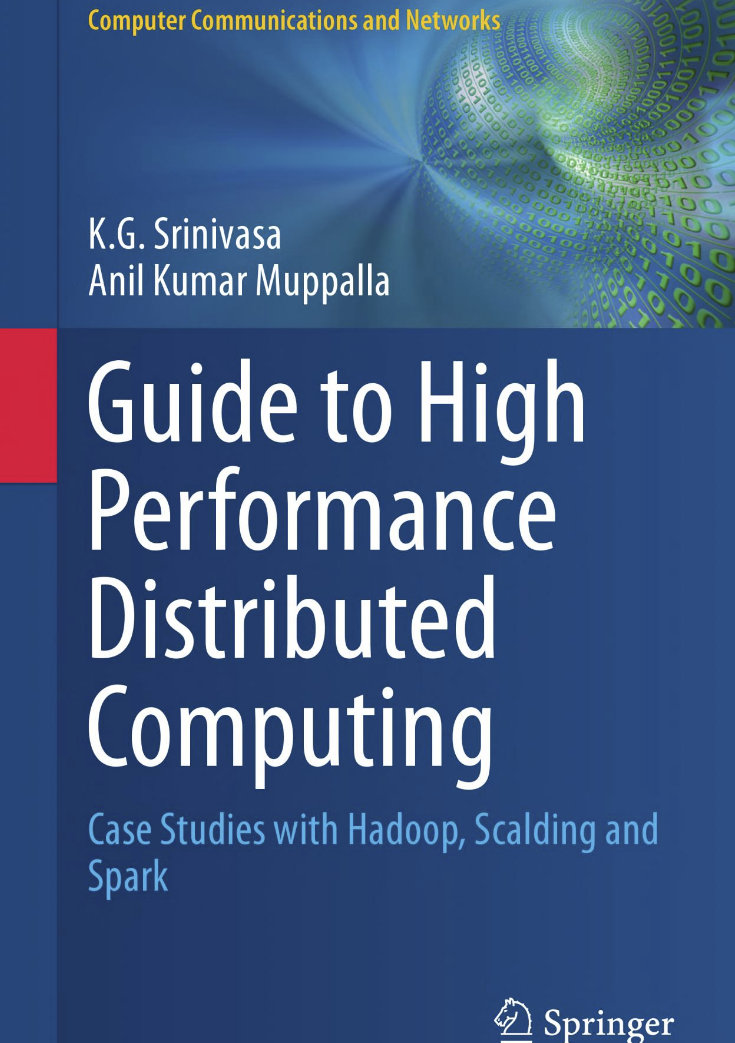
\includegraphics[width=.8\linewidth,height=.7\textheight]{./Figures/chapter-00/high-performance-computing.png}
	\end{minipage}
\end{figure}
\end{frame}

\begin{frame}[c]
\frametitle{Textbooks-2}

\begin{figure}[ht]
	\begin{minipage}[c][1\width]{0.3\textwidth}
		\centering
		
\includegraphics[width=.9\linewidth,height=.7\textheight]{./Figures/chapter-00/bjarnason.png}
	\end{minipage}
	\hfill
	\begin{minipage}[c][1\width]{0.3\textwidth}
		\centering
		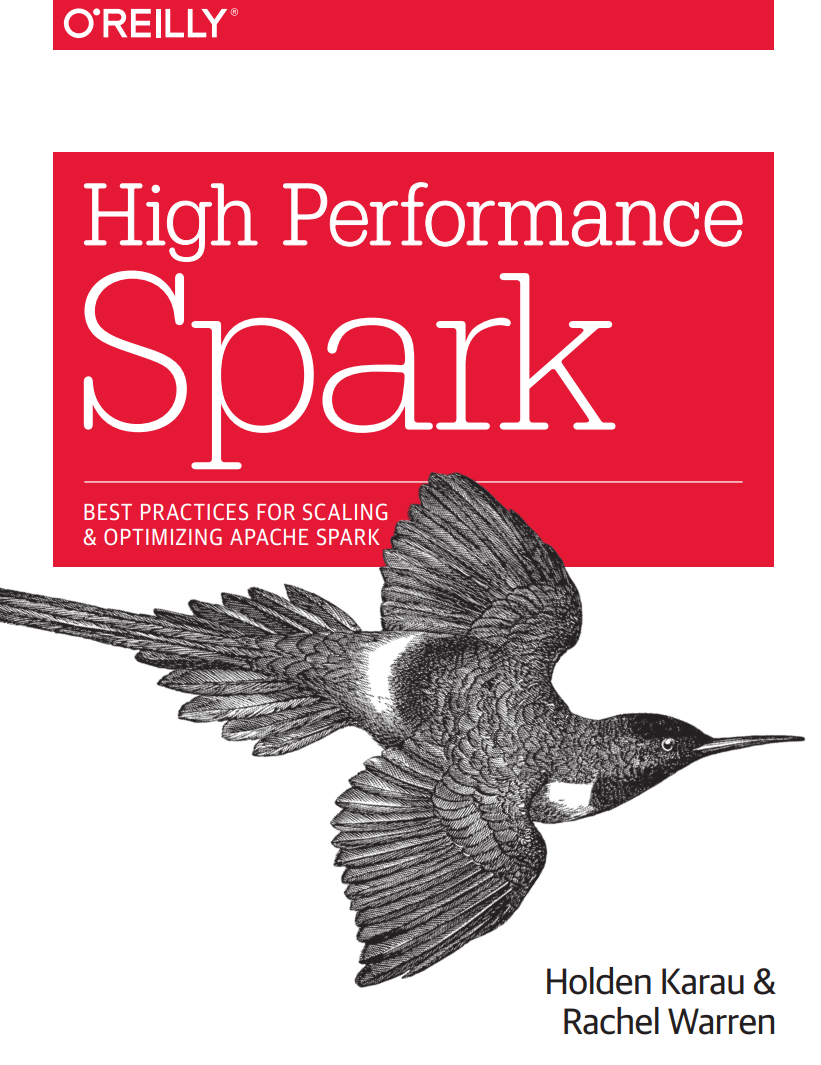
\includegraphics[width=.9\linewidth,height=.7\textheight]{./Figures/chapter-00/spark-high-performance.png}
	\end{minipage}
\hfill
	\begin{minipage}[c][1\width]{0.3\textwidth}
	\centering
	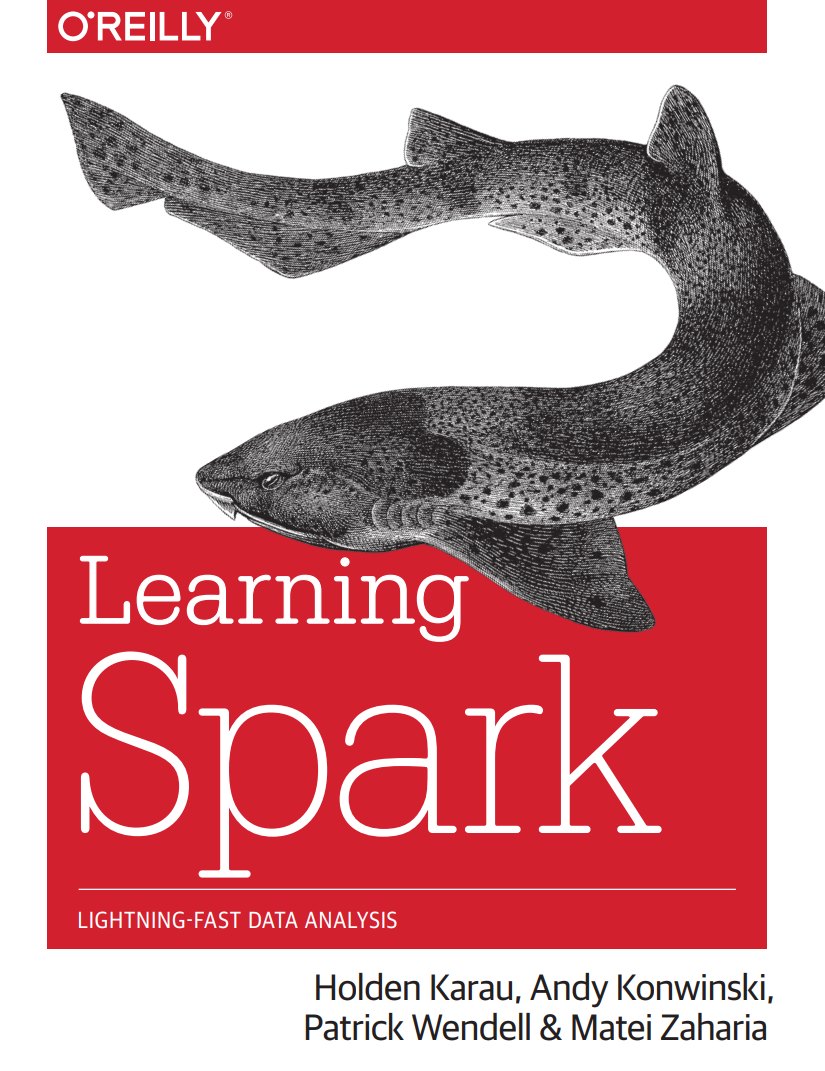
\includegraphics[width=.9\linewidth,height=.7\textheight]{./Figures/chapter-00/learning_spark_front.png}
\end{minipage}

	%	\caption{}
\end{figure}
\end{frame}

\begin{frame}[c]
	\frametitle{Textbooks-3}
	
	\begin{figure}[ht]
		\begin{minipage}[c][1\width]{0.3\textwidth}
			\centering
			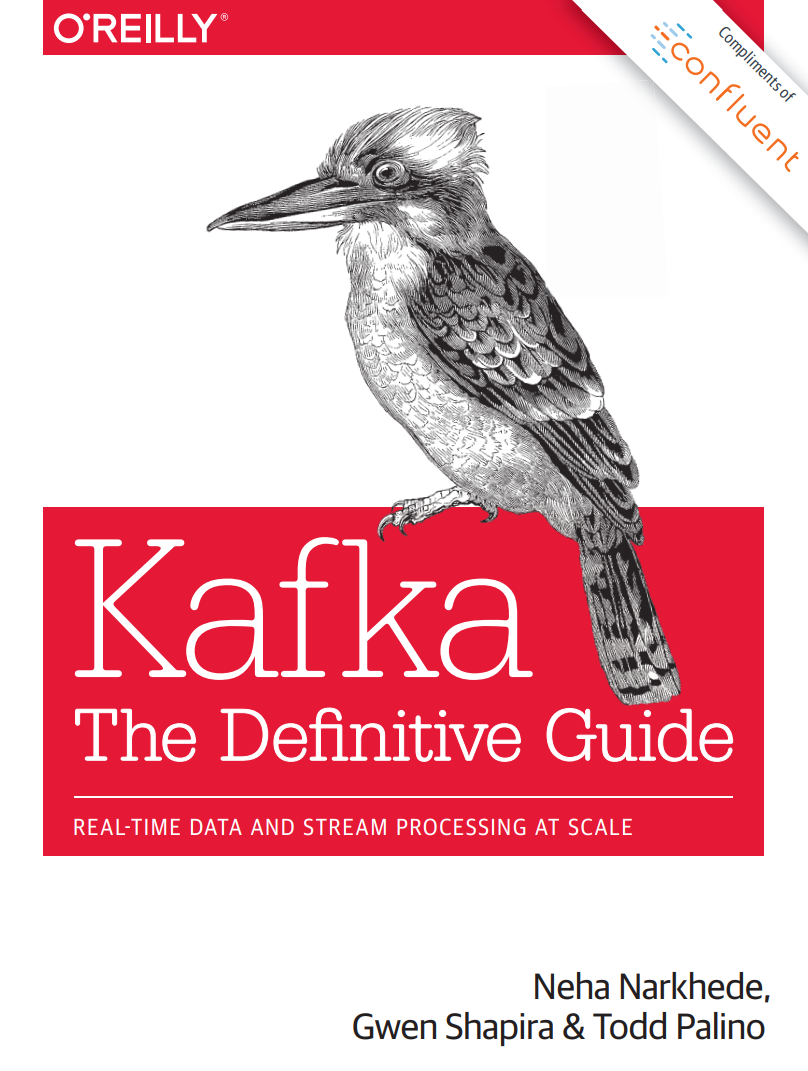
\includegraphics[width=.9\linewidth,height=.7\textheight]{./Figures/chapter-00/kafka-tdg.png}
		\end{minipage}
		\hfill	
		\begin{minipage}[c][1\width]{0.3\textwidth}
			\centering
			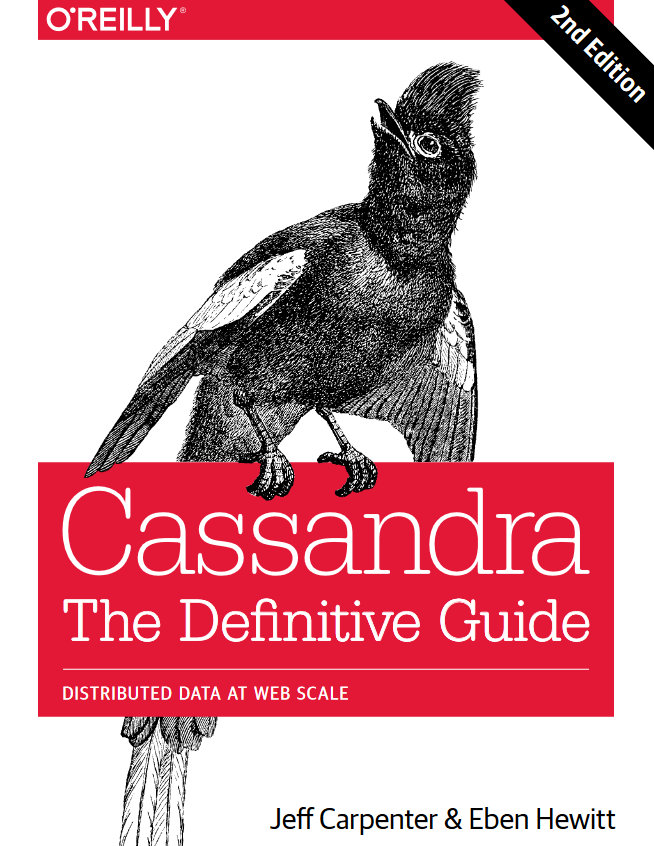
\includegraphics[width=.9\linewidth,height=.7\textheight]{./Figures/chapter-00/cassandra.png}
		\end{minipage}
		\hfill
		\begin{minipage}[c][1\width]{0.3\textwidth}
			\centering
			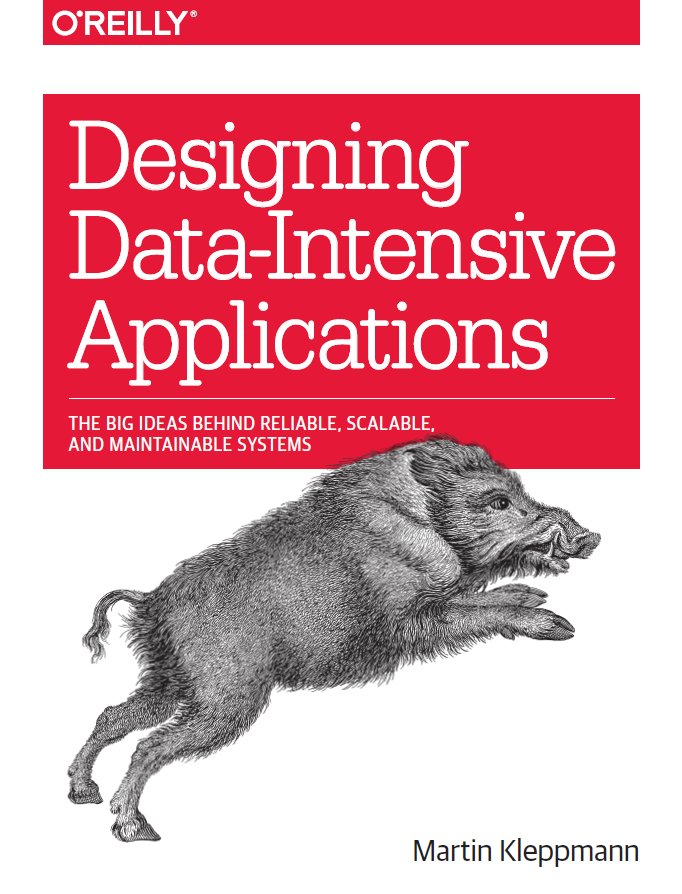
\includegraphics[width=.9\linewidth,height=.7\textheight]{./Figures/chapter-00/ddi.png}
		\end{minipage}
		
		%	\caption{}
	\end{figure}
\end{frame}


%%---------------------------------------------------------
%\begin{frame}
%	\frametitle{Videos classification}
%	
%	\begin{itemize}[<+->]
%		\item First 5 sec for every video contains a classification for this video as the following:
%		\begin{itemize}[<+->]
%			\item Length: 
%				\begin{itemize}[<+->]
%						\item Short (2:5 min).
%						\item Medium (6:12 min).
%						\item Long (12:20 min).
%				\end{itemize}
%			\item Audience: Development, DevOps, Business.
%				\begin{itemize}[<+->]
%					\item Developer.
%					\item DevOps.
%					\item Business.
%				\end{itemize}
%			\item Watching Method:
%				\begin{itemize}[<+->]
%					\item On Computer (Focus and rewrite coding).
%					\item On Mobile/Tablet (charts and points you need to watch).
%					\item Just listening (You can listen anywhere walking, driving, etc).
%				\end{itemize}
%		\end{itemize}
%	\end{itemize}
%\end{frame}

%---------------------------------------------------------
%---------------------------------------------------------
%\begin{frame}
%	\frametitle{Videos classification}
%	
%		\begin{table}[t]
%		\centering	
%%		\resizebox{\columnwidth}{!}{%
%			
%			%		\centering
%			\begin{tabular}{|c |c | c | c|}
%				\hline
%				\thead{Watching Method \\ / Audience}  & \thead{Computer} & \thead{Mobile/Tablet} &  \thead{Just 	listening} \\
%				\hline
%				\thead{Developer} & \redcircled  &   & \\
%				\hline
%				\thead{DevOps}  &  &  & \bluecircled \\
%				\hline
%				\thead{Business} &  & \greencircled & \\
%				\hline%Watching Method \newline Audience
%			\end{tabular}
%			\centering
%			\vspace{.6\baselineskip}
%			\caption{Video classification\\ The green circle \greencircled \space means short video. \\The blue circle \bluecircled \space  means medium video.\\ The red circle \redcircled \space  means long video}\label{Tab:Data_Representation_Matrix}
%	\end{table}
%\end{frame}
%---------------------------------------------------------


\begin{frame}
\frametitle{Ugly but important}

\begin{itemize}[<+->]
	\item User stories or technical discussions are not related to any of my current work or my previous companies.
	\item I am working at EPAM Systems. My company approved me for doing this online course public but the materials are not reviewed or assessed by my company. It is on my responsibilities.
\end{itemize}
\end{frame}

%---------------------------------------------------------
%\subsection{Course Textbooks}
%\begin{frame}
%\frametitle{Textbooks-1}
%\begin{itemize}
%	\item<1-> Hadoop: The Definitive Guide: Storage and Analysis at Internet Scale 4th Edition by Tom White.
%	\item<2-> Learning Spark by Matei Zaharia, Patrick Wendell, Andy Konwinski, Holden Karau
%	\item<3-> High Performance Spark Best Practices for Scaling and Optimizing Apache Spark By Holden Karau, Rachel Warren.
%	\item<4-> Kafka: The Definitive Guide by Todd Palino, Gwen Shapira, Neha Narkhede.
%	\item<5-> Guide to High Performance Distributed Computing: Case Studies with Hadoop, Scalding and Spark (Computer Communications and Networks) 2015th Edition			
%	\item<6-> Cassandra: The Definitive Guide: Distributed Data at Web Scale 2nd Edition.
%	\item<7-> Category Theory for Programmers Scala Edition By Bartosz Milewski, compiled and edited by	Igal Tabachnik.
%	\item<8-> Designing Data-Intensive Applications: The Big Ideas Behind Reliable, Scalable, and Maintainable Systems 1st Edition by Martin Kleppmann			
%	
%\end{itemize}
%\end{frame}

%\begin{frame}
%\frametitle{Sample frame title}
%This is a text in second frame. For the sake of showing an example.
%
%\begin{itemize}
%    \item<1-> Text visible on slide 1
%    \item<2-> Text visible on slide 2
%    \item<3> Text visible on slides 3
%    \item<4-> Text visible on slide 4
%\end{itemize}
%\end{frame}

%%---------------------------------------------------------
%%Example of the  command
%\begin{frame}
%In this slide 
%
%the text will be partially visible 
%
%And finally everything will be there
%\end{frame}

%\section{Second section}
%
%%---------------------------------------------------------
%%Highlighting text
%\begin{frame}
%\frametitle{Sample frame title}
%
%In this slide, some important text will be
%\alert{highlighted} beause it's important.
%Please, don't abuse it.
%
%\begin{block}{Remark}
%Sample text
%\end{block}
%
%\begin{alertblock}{Important theorem}
%Sample text in red box
%\end{alertblock}
%
%\begin{examples}
%Sample text in green box. "Examples" is fixed as block title.
%\end{examples}
%\end{frame}
%%---------------------------------------------------------
%
%
%%---------------------------------------------------------
%%Two columns
%\begin{frame}
%\frametitle{Two-column slide}
%
%\begin{columns}
%
%\column{0.5\textwidth}
%This is a text in first column.
%$$E=mc^2$$
%\begin{itemize}
%\item First item
%\item Second item
%\end{itemize}
%
%\column{0.5\textwidth}
%This text will be in the second column
%and on a second tought this is a nice looking
%layout in some cases.
%\end{columns}
%\end{frame}
%%---------------------------------------------------------

%%%%%%%%%%%%%%%%%%%%%%%%%%%%%%%%%%%%%%%%%%%%%%%%%%%%%%%%%%%%%%%%%%%%%%%%%%%
%%% Local Variables:
%%% mode: latex
%%% TeX-master: "../main"
%%% TeX-engine: xetex
%%% End:
